\documentclass{article}
\usepackage[utf8]{inputenc}

\usepackage[a4paper, total={6in, 8in}]{geometry}

\usepackage{natbib}
\bibliographystyle{plainnat}
\renewcommand{\bibsection}{\subsubsection*{References}}

\usepackage{graphicx}
\usepackage{url}

\bibliographystyle{abbrvnat}

%\usepackage[dvipsnames]{xcolor}

\usepackage{amsmath}
\usepackage{amsthm}
\usepackage{amssymb}

\DeclareMathOperator*{\argmax}{argmax}

\title{The Causal Health Classification Data set}
\author{}
\date{} % no date

\begin{document}

\maketitle


The causal health classification data set is an extension to the causal health data set by \cite{Zecevic2021a}, where three new binary "Diagnosis" variables, in a one-hot configuration, are introduced. In this case one of the diagnose variables is set to true and the remaining ones are set to false for every data point.

\begin{figure}[h]
\centering
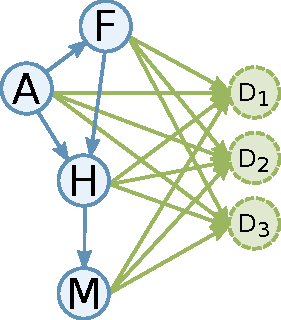
\includegraphics[width=0.2\linewidth]{figure_CHCDAG.pdf}
\caption{The DAG of the structural causal model of the Causal Health Classification Data set. Variables of the already existing Causal Health data set (blue) with the new diagnosis variables (green/dashed) added. (Best viewed in color.)}
\label{SCMCHC}
\end{figure}

For each sample three multivariate polynomial functions are evaluated to determine the activate diagnose. Each function which depends on a subset of the original variables $A, M, F$ and $H$:
\[
\begin{split}
  & f_1(A) :=
  \begin{cases}
    0.00108 A^3 - 0.08862 A^2 + 1.337 A + \mathcal{N}(25, 10) & \text{if } A\leq4.09837\\
     \mathcal{N}(5, 10),              & \text{otherwise}
  \end{cases} \\
  & f_2(F,M) := 0.0175F + 0.525M + \mathcal{N}(0, 5) \\
  & f_3(A,H) := 0.00013857 A^3 - 0.0135 A^2 + 0.2025 A + 0.2025 H + \mathcal{N}(17.1714, 0.2A)
\end{split}
\]

The state of each diagnose variable $D_i$ is determined by taking the argmax over all three functions.
\[
  f_{Di}(A, F, H, M) :=
  \begin{cases}
    \mathit{true} & \text{if} \argmax(f_1(A), f_2(M,F), f_3(A,H)) = i \\
    \mathit{false} & \text{otherwise}
  \end{cases}
\]


The resulting SCM, as shown in Figure~\ref{SCMCHC}, consists of the Causal Health SCM with three additional Diagnose variables. Connections from $A, F, H$ and $M$ to every $D_i$ are introduced, since $f_{Di}(A, F, H, M)$ depends on all four original variables.

All interventions are carried out to be perfectly atomic, while every intervention sets the affected variable to a uniform distribution.

%\section*{References}
\bibliography{CausalHealthClassificationRefs}

\end{document}
